\documentclass[9pt]{beamer}
\usepackage[utf8]{inputenc}
\usepackage[english]{babel}
\usepackage{amssymb, amsmath, amsthm, amsfonts, amscd, graphicx,
            array, multicol, setspace, caption, color, tikz, listings}
\usetikzlibrary{intersections, decorations.pathmorphing,
                shapes.geometric, arrows.meta, positioning, backgrounds}
\usepackage{pifont}
\usepackage{textcomp}
\usepackage{colortbl}
\usepackage{fix-cm}
\usepackage{csquotes}
%----------------------------------------------
\usecolortheme{beaver}
\usetheme{Frankfurt}
\setbeamercolor{section in head/foot}{bg=black}
\setbeamercolor{title}{fg=white, bg=black}
\setbeamercolor{frametitle}{fg=white, bg=black}
\setbeamercolor{block title}{fg=white, bg=black}
\setbeamercolor{block body}{bg=gray!15}
\setbeamercolor{item}{fg=gray}
\setbeamertemplate{navigation symbols}{}
\setbeamercovered{transparent}
%----------------------------------------------
% Kod stili
\lstdefinestyle{arduino}{
  basicstyle=\ttfamily\tiny\color{white},
  backgroundcolor=\color{black!85},
  keywordstyle=\color{yellow!80}\bfseries,
  commentstyle=\color{green!60}\itshape,
  stringstyle=\color{orange!80},
  language=C++,
  breaklines=true,
  frame=single, framerule=0pt,
  numbers=left, numberstyle=\tiny\color{gray},
  xleftmargin=1.5em, framexleftmargin=1em,
  tabsize=2, showstringspaces=false,
}
%----------------------------------------------
\newcommand{\mysection}[1]{\section{#1}\def\sectionname{#1}\SectionFrame}
%----------------------------------------------
\newcommand{\Front}{%
  \thispagestyle{empty}
  \begin{frame}
    \begin{figure}
      \centering
      
\includegraphics[width=0.25\textwidth]{Logos/SUT.png}
    \end{figure}
    \maketitle
  \end{frame}
}
\newcommand{\overview}{%
  \begin{frame}{Genel Bakis}
    \tableofcontents
  \end{frame}
}
\newcommand{\SectionFrame}{%
  \begin{frame}{}
    \begin{center}
      {\fontsize{25pt}{36pt}\selectfont \thesection.\ \sectionname}
    \end{center}
  \end{frame}
}
\newcommand{\Ending}[1]{%
  \begin{frame}{}
    \begin{center}
      {\fontsize{35pt}{36pt}\selectfont #1}
    \end{center}
  \end{frame}
}

\title[Veri Toplayici v2]{Sensor Verisi Kaydeden\\Mini Veri Toplayici}
\author[Ogrenci]{Ogrenci Adi \texorpdfstring{\\}{} [1ex]
  {\small Ders: Mikrodenetleyici Sistemleri}}
\institute[Universite]{Elektrik--Elektronik Muhendisligi Bolumu}
\date[]{2026}

\begin{document}
\Front
\overview
%----------------------------------------------
\mysection{Proje Tanimi}
\subsection{Amac ve Gereksinimler}
\begin{frame}{Amac ve Gereksinimler}
  \begin{columns}[T]
    \column{0.48\textwidth}
      \begin{block}{Zorunlu Gereksinimler}
        \begin{itemize}
          \item Sensor verisi \textbf{belirli araliklarla} okunur
          \item Veriler \textbf{zaman bilgisiyle} kaydedilir
          \item Reset'te onceki veriler \textbf{korunur}
        \end{itemize}
      \end{block}
      \vspace{6pt}
      \begin{block}{Genisl. (Bonus)}
        \begin{itemize}
          \item Maksimum / minimum deger kaydi
          \item Alarm esigi olusturma
          \item Butonla ozet rapor
          \item LED gorsel alarm
        \end{itemize}
      \end{block}

    \column{0.48\textwidth}
      \begin{block}{Proje Ozeti}
        \begin{itemize}
          \item \textbf{2 sensor:} LM35 + LDR
          \item \textbf{Kayit:} SD kart (veri.csv)
          \item \textbf{Zaman:} Uptime sayaci
          \item \textbf{Rapor:} ozet.txt (butona bas)
          \item \textbf{Alarm:} 4 farkli esik
          \item \textbf{Platform:} Arduino Uno/Nano
        \end{itemize}
      \end{block}
      \vspace{6pt}
      \begin{alertblock}{Sonuc}
        \small Tum zorunlu gereksinimler \textbf{ve}
        tum bonus ozellikler karsilanmistir.
      \end{alertblock}
  \end{columns}
\end{frame}

\subsection{Donanim}
\begin{frame}{Donanim ve Baglanti Semaasi}
  \begin{columns}[T]
    \column{0.38\textwidth}
      \begin{block}{Malzeme Listesi}
        \begin{tabular}{ll}
          \textbf{MCU}      & Arduino Uno \\
          \textbf{Sensor 1} & LM35 (sicaklik) \\
          \textbf{Sensor 2} & LDR (isik) \\
          \textbf{Depolama} & SD Kart Mod. \\
          \textbf{Giris}    & Buton (D2) \\
          \textbf{Cikis}    & LED (D13) \\
        \end{tabular}
      \end{block}
      \vspace{4pt}
      \begin{block}{Pin Baglantilari}
        \scriptsize
        \begin{tabular}{ll}
          \texttt{D10} & SD -- CS \\
          \texttt{D11} & SD -- MOSI \\
          \texttt{D12} & SD -- MISO \\
          \texttt{D13} & SD -- SCK / LED \\
          \texttt{A0}  & LDR \\
          \texttt{A5}  & LM35 \\
          \texttt{D2}  & Buton \\
        \end{tabular}
      \end{block}

    \column{0.58\textwidth}
      \begin{block}{Baglanti Semasi}
        \begin{center}
        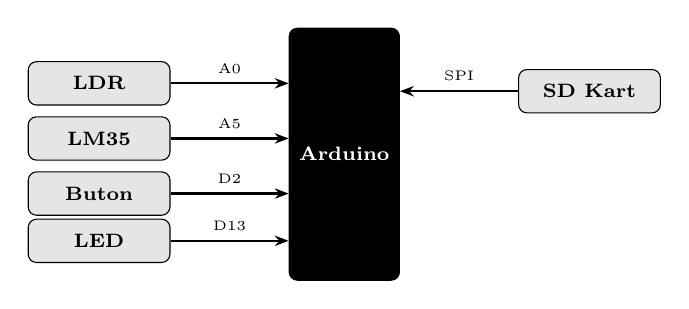
\begin{tikzpicture}[
          box/.style={rectangle, draw=black, fill=gray!20,
                      rounded corners=3pt, minimum width=1.8cm,
                      minimum height=0.55cm, font=\scriptsize\bfseries,
                      text centered},
          arr/.style={-{Stealth[length=5pt]}, thick},
          node distance=0.4cm and 1.3cm,
        ]
          \node[box, fill=black, text=white, minimum height=3.2cm,
                minimum width=1.4cm] (ard) {Arduino};

          \node[box, right=1.5cm of ard, yshift= 0.8cm] (sd)  {SD Kart};
          \node[box, left =1.5cm of ard, yshift= 0.9cm] (ldr) {LDR};
          \node[box, left =1.5cm of ard, yshift= 0.2cm] (lm)  {LM35};
          \node[box, left =1.5cm of ard, yshift=-0.5cm] (btn) {Buton};
          \node[box, left =1.5cm of ard, yshift=-1.1cm] (led) {LED};

          \draw[arr] (sd.west)  -- node[above,font=\tiny]{SPI} (ard.east |- sd);
          \draw[arr] (ldr.east) -- node[above,font=\tiny]{A0}  (ard.west |- ldr);
          \draw[arr] (lm.east)  -- node[above,font=\tiny]{A5}  (ard.west |- lm);
          \draw[arr] (btn.east) -- node[above,font=\tiny]{D2}  (ard.west |- btn);
          \draw[arr] (led.east) -- node[above,font=\tiny]{D13} (ard.west |- led);
        \end{tikzpicture}
        \end{center}
      \end{block}
  \end{columns}
\end{frame}

%----------------------------------------------
\mysection{Yazilim Mimarisi}
\subsection{Modul Yapisi}
\begin{frame}{Modul Yapisi -- Katmanli Mimari}
  \begin{center}
  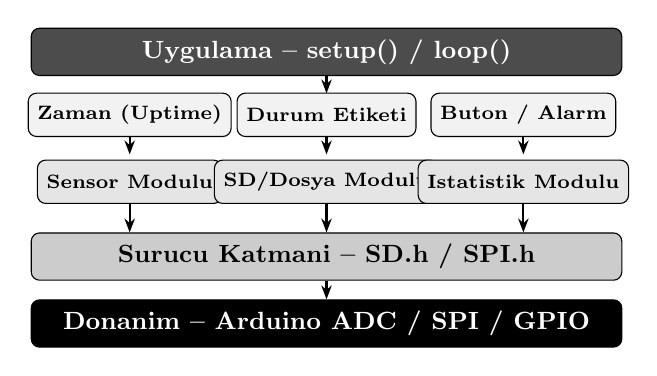
\begin{tikzpicture}[
    layer/.style={rectangle, draw=black, minimum width=7.5cm,
                  minimum height=0.6cm, rounded corners=3pt,
                  font=\small\bfseries, text centered},
    mod/.style={rectangle, draw=black, fill=gray!20, rounded corners=3pt,
                minimum width=2.1cm, minimum height=0.55cm,
                font=\scriptsize\bfseries, text centered},
    arr/.style={-{Stealth[length=5pt]}, thick},
  ]
    % Katmanlar (aşağıdan yukarı)
    \node[layer, fill=black, text=white] (hw)
      at (0,0) {Donanim -- Arduino ADC / SPI / GPIO};

    \node[layer, fill=gray!40] (drv)
      at (0,0.85) {Surucu Katmani -- SD.h / SPI.h};

    % Modül satırı
    \node[mod] (ms) at (-2.5, 1.8) {Sensor Modulu};
    \node[mod] (mf) at ( 0.0, 1.8) {SD/Dosya Modulu};
    \node[mod] (mi) at ( 2.5, 1.8) {Istatistik Modulu};

    % Yardımcı modüller
    \node[mod, fill=gray!10] (mu) at (-2.5, 2.65) {Zaman (Uptime)};
    \node[mod, fill=gray!10] (md) at ( 0.0, 2.65) {Durum Etiketi};
    \node[mod, fill=gray!10] (mb) at ( 2.5, 2.65) {Buton / Alarm};

    % Uygulama katmanı
    \node[layer, fill=black!70, text=white] (app)
      at (0,3.45) {Uygulama -- setup() / loop()};

    % Oklar
    \foreach \m in {ms,mf,mi}
      \draw[arr] (\m.south) -- (drv.north -| \m);
    \foreach \m in {mu,md,mb}
      \draw[arr] (\m.south) -- ++(0,-0.22);
    \draw[arr] (drv.south) -- (hw.north);
    \draw[arr] (app.south) -- ++(0,-0.22);
  \end{tikzpicture}
  \end{center}
\end{frame}

\subsection{Fonksiyonlar}
\begin{frame}{Fonksiyon Tablosu}
  \begin{center}
  \small
  \begin{tabular}{|l|l|p{5.5cm}|}
    \hline
    \rowcolor{black}\color{white}\textbf{Fonksiyon} &
    \color{white}\textbf{Donus} &
    \color{white}\textbf{Gorev} \\
    \hline
    \texttt{uptimeStr()} & \texttt{void} &
      Global \texttt{uptimeBuf[]} alanina GGG-SS:DD:SN yazar \\
    \hline
    \rowcolor{gray!15}
    \texttt{sicaklikOku()} & \texttt{float} &
      8 ornek ortalamasi ile LM35'ten \textcelsius{} okur \\
    \hline
    \texttt{ldrOku()} & \texttt{int} &
      4 ornek ortalamasi ile LDR degeri okur \\
    \hline
    \rowcolor{gray!15}
    \texttt{durumEtiket()} & \texttt{void} &
      Alarm durumlarini \texttt{durumBuf[]} alanina yazar \\
    \hline
    \texttt{csvYaz()} & \texttt{void} &
      \texttt{veri.csv} dosyasina satir ekler \\
    \hline
    \rowcolor{gray!15}
    \texttt{ozetYaz()} & \texttt{void} &
      \texttt{ozet.txt} ozet raporunu olusturur \\
    \hline
    \texttt{setup()} & --- &
      Donanim ve SD kart baslatma \\
    \hline
    \rowcolor{gray!15}
    \texttt{loop()} & --- &
      Buton kontrolu + periyodik kayit dongusu \\
    \hline
  \end{tabular}
  \end{center}
\end{frame}

%----------------------------------------------
\mysection{Algoritma ve Veri}
\subsection{Ana Dongü Akisi}
\begin{frame}{Ana Dongu Akis Diyagrami}
  \begin{columns}[T]
    \column{0.48\textwidth}
    \begin{center}
    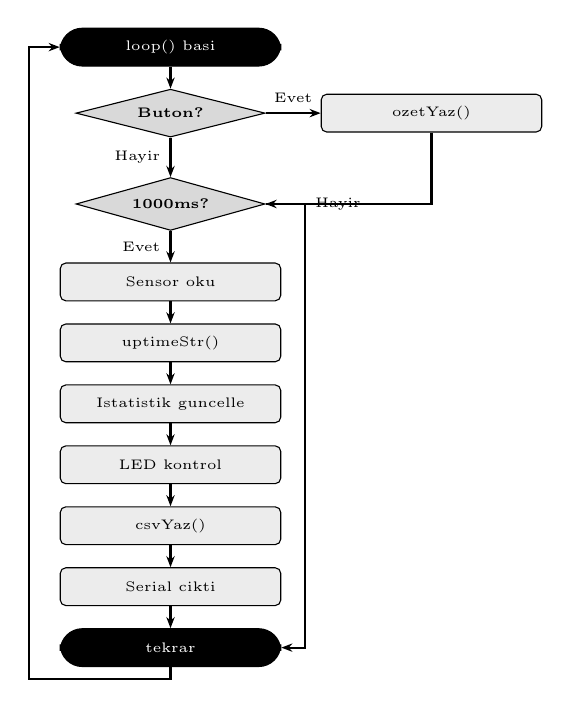
\begin{tikzpicture}[
      proc/.style={rectangle, draw=black, fill=gray!15,
                   rounded corners=2pt, minimum width=2.8cm,
                   minimum height=0.48cm, font=\tiny, text centered},
      dec/.style={diamond, draw=black, fill=gray!30, aspect=2.2,
                  minimum width=2.4cm, font=\tiny\bfseries, inner sep=1pt},
      term/.style={proc, fill=black, text=white, rounded corners=8pt},
      arr/.style={-{Stealth[length=4pt]}, thick},
      node distance=0.28cm,
    ]
      \node[term] (s)  {loop() basi};
      \node[dec,  below=of s]  (b)  {Buton?};
      \node[proc, right=0.7cm of b] (oz) {ozetYaz()};
      \node[dec,  below=0.5cm of b] (t)  {1000ms?};
      \node[proc, below=0.4cm of t] (ok) {Sensor oku};
      \node[proc, below=0.28cm of ok](up) {uptimeStr()};
      \node[proc, below=0.28cm of up](st) {Istatistik guncelle};
      \node[proc, below=0.28cm of st](ld) {LED kontrol};
      \node[proc, below=0.28cm of ld](cs) {csvYaz()};
      \node[proc, below=0.28cm of cs](se) {Serial cikti};
      \node[term, below=0.28cm of se](e)  {tekrar};

      \draw[arr] (s)--(b);
      \draw[arr] (b)--node[left,font=\tiny]{Hayir}(t);
      \draw[arr] (b)--node[above,font=\tiny]{Evet}(oz);
      \draw[arr] (oz)|-(t);
      \draw[arr] (t)--node[left,font=\tiny]{Evet}(ok);
      \draw[arr] (t.east)--++(0.5,0)node[right,font=\tiny]{Hayir}|-(e.east);
      \draw[arr] (ok)--(up);
      \draw[arr] (up)--(st);
      \draw[arr] (st)--(ld);
      \draw[arr] (ld)--(cs);
      \draw[arr] (cs)--(se);
      \draw[arr] (se)--(e);
      \draw[arr] (e.south)--++(0,-0.15)-|++(-1.8,0)|-(s.west);
    \end{tikzpicture}
    \end{center}

    \column{0.48\textwidth}
      \begin{block}{millis() Tabanli Zamanlama}
        \small
        \texttt{delay()} kullanilmaz!\\[4pt]
        \texttt{if (simdi - sonKayit >= 1000)}\\[4pt]
        \begin{itemize}\small
          \item Buton her an algilanir
          \item Kayit tam 1 saniyede bir olur
          \item Sensor okuma \textbf{bloklamaz}
        \end{itemize}
      \end{block}
      \vspace{6pt}
      \begin{block}{Buton Debounce}
        \small
        \begin{enumerate}
          \item Dusus kenari algilanir\\
                (HIGH $\to$ LOW)
          \item 30ms beklenir
          \item Pin tekrar okunur
          \item Hala LOW ise gecerli
        \end{enumerate}
      \end{block}
  \end{columns}
\end{frame}

\subsection{Bellek Optimizasyonu}
\begin{frame}{Bellek Optimizasyonu -- Arduino Uno: 2KB RAM}
  \begin{columns}[T]
    \column{0.48\textwidth}
      \begin{block}{Sorun: String Nesneleri}
        \small
        \texttt{String} sinifi heap'i \textbf{parcalar}:
        \begin{itemize}
          \item Dinamik bellek tahsisi
          \item Heap parcalanmasi
          \item SD baslatma icin yer kalmaz
          \item[\ding{55}] SD kart hatalari
        \end{itemize}
      \end{block}
      \vspace{6pt}
      \begin{block}{Cozum: char{[}{]} + F()}
        \small
        \begin{itemize}
          \item[\ding{51}] \texttt{char uptimeBuf[20]}
          \item[\ding{51}] \texttt{char durumBuf[40]}
          \item[\ding{51}] \texttt{F("sabit metin")}
          \item[] Sabit metinler Flash'a tasindi
          \item[] $\approx$400--500 byte RAM kazanildi
        \end{itemize}
      \end{block}

    \column{0.48\textwidth}
      \begin{block}{Sensor Gürültu Azaltma}
        \small
        \textbf{LM35:} 8 ornek ortalamasi
        \[ T = \frac{1}{8}\sum_{i=1}^{8} x_i \cdot \frac{V_{ref}}{1023} \cdot 100 \]
        Standart sapma $\sigma \to \sigma/\sqrt{8}$\\[6pt]
        \textbf{LDR:} 4 ornek ortalamasi
        \[ L = \frac{1}{4}\sum_{i=1}^{4} x_i \]
      \end{block}
      \vspace{6pt}
      \begin{alertblock}{Kritik Not}
        \small \texttt{F()} makrosu olmadan buyuk
        kodlarda RAM dolarak program kilitleniyor.
      \end{alertblock}
  \end{columns}
\end{frame}

\subsection{Alarm Sistemi}
\begin{frame}{Alarm Sistemi}
  \begin{columns}[T]
    \column{0.52\textwidth}
      \begin{block}{Alarm Esikleri}
        \begin{center}
        \small
        \begin{tabular}{|l|c|l|}
          \hline
          \rowcolor{black}\color{white}\textbf{Durum} &
          \color{white}\textbf{Kosul} &
          \color{white}\textbf{Etiket} \\
          \hline
          Asiri Sicak & $T \geq 35$\textcelsius & \texttt{SICAK\_ALARM} \\
          \hline
          \rowcolor{gray!15}
          Asiri Soguk & $T \leq 10$\textcelsius & \texttt{SOGUK\_ALARM} \\
          \hline
          Karanlik    & LDR $\leq 200$ & \texttt{KARANLIK} \\
          \hline
          \rowcolor{gray!15}
          Cok Parlak  & LDR $\geq 900$ & \texttt{COK\_PARLAK} \\
          \hline
          Normal      & Hicbiri & \texttt{Normal} \\
          \hline
        \end{tabular}
        \end{center}
      \end{block}
      \vspace{4pt}
      \begin{block}{Birden Fazla Alarm}
        \small
        Kosullar \texttt{|} ile birlestirilir:\\
        \texttt{SICAK\_ALARM|KARANLIK}
      \end{block}

    \column{0.44\textwidth}
      \begin{block}{LED Alarm Gostergesi}
        \small
        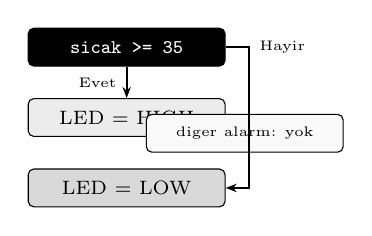
\begin{tikzpicture}[
          node distance=0.4cm,
          box/.style={rectangle, draw=black, fill=gray!15,
                      rounded corners=2pt, minimum width=2.5cm,
                      minimum height=0.48cm, font=\scriptsize, text centered},
          arr/.style={-{Stealth[length=4pt]}, thick},
        ]
          \node[box, fill=black, text=white] (c) {\texttt{sicak >= 35}};
          \node[box, below=of c] (y) {LED = HIGH};
          \node[box, below=of y, fill=gray!30] (n) {LED = LOW};
          \node[box, below=0.6cm of c, xshift=1.5cm, fill=gray!5,
                font=\tiny] (e) {diger alarm: yok};
          \draw[arr] (c)--node[left,font=\tiny]{Evet}(y);
          \draw[arr] (c.east)--++(0.3,0)node[right,font=\tiny]{Hayir}|-(n.east);
        \end{tikzpicture}
      \end{block}
      \vspace{4pt}
      \begin{block}{Istatistik Sayaclari}
        \scriptsize
        \texttt{sicakAlarm++} $\leftarrow$ her asim\\
        \texttt{karanlikAlarm++} $\leftarrow$ her karanlik\\
        Ozet raporunda gosterilir.
      \end{block}
  \end{columns}
\end{frame}

%----------------------------------------------
\mysection{Ciktilar}
\subsection{Dosya Yapisi}
\begin{frame}{SD Kart Dosya Yapisi}
  \begin{columns}[T]
    \column{0.50\textwidth}
      \begin{block}{\texttt{veri.csv} -- Surekli Kayit}
        \scriptsize
        \texttt{FILE\_WRITE} modu: \textbf{ekleme yapar}\\[4pt]
        \begin{tabular}{|l|}
          \hline
          \texttt{No,Uptime,Sicaklik,LDR\_Ham,...}\\
          \texttt{1,000-00:00:01,24.50,512,...}\\
          \texttt{2,000-00:00:02,35.10,150,...}\\
          \hline
        \end{tabular}
        \vspace{4pt}
        \begin{itemize}
          \item Ilk satir bos ise baslik yazar
          \item Reset sonrasi veriler \textbf{korunur}
          \item Her saniye 1 satir eklenir
        \end{itemize}
      \end{block}

    \column{0.46\textwidth}
      \begin{block}{\texttt{ozet.txt} -- Rapor}
        \scriptsize
        Butona basilinca \textbf{sifirdan} yazilir:\\[4pt]
        \begin{tabular}{|l|}
          \hline
          \texttt{Toplam kayit : 932}\\
          \texttt{Sicak Max    : 37.20 C}\\
          \texttt{Sicak Min    : 22.10 C}\\
          \texttt{Sicak Ort    : 25.43 C}\\
          \texttt{Sicak alarm  : 14}\\
          \texttt{LDR Max      : 980 (95\%)}\\
          \texttt{Karanlik al. : 3}\\
          \hline
        \end{tabular}
      \end{block}
      \vspace{4pt}
      \begin{alertblock}{SD Kart Gereksinimleri}
        \scriptsize
        FAT32 formatlanmis $\cdot$ 32GB alti\\
        SPI protokolü (D10--D13)
      \end{alertblock}
  \end{columns}
\end{frame}

\subsection{Ornek Cikti}
\begin{frame}[fragile]{Serial Monitor Ciktisi ve Kod Ornegi}
  \begin{block}{Serial Monitor -- Her 15 Satirda Baslik Tekrar}
    \scriptsize\ttfamily
    \begin{tabular}{l|l|l|l|l|l}
      No & Uptime & Sicak & LDR & \%Isik & Durum \\
      \hline
      1 & 000-00:00:01 & 24.50 C & 512 & 50\% & Normal \\
      2 & 000-00:00:02 & 24.52 C & 156 & 15\% & KARANLIK \\
      3 & 000-00:00:03 & 35.10 C & 156 & 15\% & SICAK\_ALARM|KARANLIK \\
    \end{tabular}
  \end{block}
  \vspace{4pt}
  \begin{block}{Temel Kayit Dongusu}
    \begin{lstlisting}[style=arduino]
if (simdi - sonKayit >= KAYIT_MS) {
    sonKayit = simdi;
    kayitNo++;
    float sicak = sicaklikOku(); // 8 ornek ort.
    int   ldr   = ldrOku();     // 4 ornek ort.
    uptimeStr();   // uptimeBuf[] guncelle
    durumEtiket(sicak, ldr); // durumBuf[] guncelle
    if (sicak > stat.sicakMax) stat.sicakMax = sicak;
    stat.say++;
    if (sdHazir) csvYaz(kayitNo, sicak, ldr);
    Serial.println(durumBuf);
}
    \end{lstlisting}
  \end{block}
\end{frame}

%----------------------------------------------
\pagestyle{empty}
\Ending{Tesekkurler}
\end{document}
